\documentclass[kapital_02.tex]{subfiles}

\begin{document}

Posamezne oznake za obliko kapitala.

D

D'%matematična črtica

Inline odnos (sosledje) v procesu.

D---B

B \dots D

Račun med količinami (med oznakami za količine, ki nastopajo v procesu).%+ in = in krat (x) (str. 205)

D+b

Odnos v procesu, ki potencialno (vertikalno) presega vrstico.
%primer na str. 438

B<\rlap{\textsuperscript{Ds}}\textsubscript{Ps}

tekst teksttekst tekst tekst tekst tekst tekst tekst tekst tekst tekst tekst tekst tekst tekst tekst tekst tekst tekst tekst tekst tekst tekst tekst tekst tekst tekst tekst tekst tekst tekst tekst tekst tekst tekst tekst tekst tekst tekst tekst tekst tekst tekst tekst tekst tekst tekst tekst tekst tekst tekst tekst tekst tekst tekst tekst tekst tekst tekst tekst tekst tekst tekst tekst tekst tekst tekst tekst tekst tekst tekst tekst tekst tekst tekst tekst tekst tekst tekst tekst tekst tekst tekst tekst tekst tekst tekst in zdaj
\(
\B
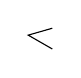
\begin{tikzpicture}[baseline=-0.33\baselineskip]
    {
        \draw[-]
            (0.87em,0.25em) --
            (0,0) --
            (0.87em,-0.5em);
    }
\end{tikzpicture}
^{\Ds}_{Ps}
\); tekst tekst  tekst tekst tekst tekst tekst tekst tekst tekst tekst tekst tekst tekst tekst tekst tekst tekst tekst tekst tekst tekst tekst tekst tekst tekst tekst tekst tekst tekst tekst tekst tekst tekst tekst tekst tekst tekst tekst tekst tekst tekst tekst tekst tekst tekst tekst tekst tekst tekst tekst tekst tekst tekst tekst tekst tekst tekst tekst tekst tekst tekst tekst tekst tekst tekst tekst tekst tekst tekst tekst tekst tekst tekst tekst tekst tekst tekst tekst tekst tekst tekst tekst tekst tekst tekst

Denarne vsote.
%fšt i tako

Horizontalni spodnji in zgornji oklepaji.

%primer na str. 69
%primer na str. 93

Matrica odnosov/sosledij.

%primer na str. 73
%primer na str. 123

Decimalna vejica pri denarnih in fizikalnih količinah. %vprašanje tudi glede merskih enot

Tabelarni pregled.

%primer na str. 100

Array procesov.

%primer na str. 111

Ulomki.

%primer na str. 172
%primer na str. 195

Tabelarni array. Razpredelnice.

%primer na str. 199
%primer na str. 207
%primer na str. 297

Naštevanje v odstavkih.

%primer na str. 253

\end{document}